\documentclass[draft,12pt,headsepline,footsepline,paper=letter]{scrreprt}
\pagestyle{headings}

\usepackage[utf8]{inputenc}
\usepackage[T1]{fontenc}
\def\spanishoptions{es-noquoting,es-nolists,mexico-com}
\usepackage[spanish]{babel}

\usepackage{makeidx}
\makeindex

\usepackage[nonumberlist]{glossaries}
\makeglossaries

\usepackage[final]{graphicx}
\DeclareGraphicsExtensions{.pdf,.png,.jpg}
\graphicspath{{media/}}

\iftrue % outline for images
\usepackage{scrhack}
\usepackage{float}
\floatstyle{boxed}
\restylefloat{figure}
\fi

\usepackage{natbib}
\usepackage{amsmath,amssymb, bm}
\usepackage{enumerate}
\usepackage{ragged2e}

\usepackage{setspace}
\onehalfspacing
\frenchspacing
\recalctypearea

\usepackage{pdfsync}

% Glossary
\newglossaryentry{asignatura} {
	   name = asignatura,
    description = {Materia que se enseña en un curso y que forma parte de un programa de estudios}}
\newglossaryentry{aula} {
	   name = aula,
    description = {Sala de un centro de enseñanza donde se imparten clases}}
\newglossaryentry{calendario} {
    name        = calendario,
    description = {Plan ordenado del conjunto de las actividades previstas durante un período}}
\newglossaryentry{calendarizacion} {
           name = calendarización,
    description = {Acción y efecto de calendarizar}}
\newglossaryentry{calendarizar} {
           name = calendarizar,
    description = {Establecer un calendario ordenado de actividades previstas}}
\newglossaryentry{catedra} {
           name = cátedra,
    description = {Aula en la que se enseña una asignatura}}
\newglossaryentry{clase} {
           name = clase,
    description = {Conjunto de escolares o estudiantes de un mismo nivel o que estudian la misma asignatura, y que asisten juntos a las lecciones correspondientes}}
\newglossaryentry{conferenciante} {
           name = conferenciante,
    description = {Persona que pronuncia una conferencia}}
\newglossaryentry{curriculo} {
           name = currículo,
    description = {Plan de estudios}}
\newglossaryentry{curso} {
           name = curso,
    description = {Conjunto de lecciones o clases sobre una materia que está estructurada y sigue un programa, especialmente dentro de un plan de estudios}}
\newglossaryentry{educacional} {
           name = educacional,
    description = {Perteneciente o relativo a la educación}}
\newglossaryentry{escuela} {
           name = escuela,
    description = {Institución o establecimiento destinados a enseñar determinadas materias especializadas}}
\newglossaryentry{factible} {
           name = factible,
    description = {Que se puede hacer}}
\newglossaryentry{horario} {
           name = horario,
    description = {Distribución de las horas en que se realiza una actividad o trabajo o se presta un servicio}}
\newglossaryentry{leccion} {
           name = lección,
    description = {Sesión docente en la que el profesor de una materia imparte un conjunto articulado de conocimientos}}
\newglossaryentry{limitacion} {
           name = limitación,
    description = {Circunstancia o condición de algo o de alguien que limita, impide o dificulta su desarrollo}}
\newglossaryentry{prevalente} {
           name = prevalente,
    description = {Que prevalece o sobresale}}
\newglossaryentry{programacion} {
           name = planificación,
    description = {Acción de programar}}
\newglossaryentry{programar} {
           name = programar,
    description = {Establecer o planificar el programa de una serie de actividades}}
\newglossaryentry{turno} {
           name = turno,
    description = {Conjunto de trabajadores que desempeñan su actividad al mismo tiempo, según un orden establecido previamente}}

\newacronym[longplural=Frames per Second]{fpsLabel}
{FPS}{Frame per Second}


\begin{document}

\title{Planificación de horarios educacionales}
\author{Héctor Arciga}
\date{\today}

\maketitle


\begin{abstract}
 
\end{abstract}

\iffalse
University timetabling represents a difficult optimisation problem and finding a high quality timetable is a challenging task. With a large number of events involved and various hard constraints to be fulfilled, finding an optimal timetable is complicated and time consuming. Many approaches in the literature have addressed this problem.
\fi

\begin{spacing}{1}
\tableofcontents
\glsaddall 
\printglossaries
\listoffigures
\listoftables
\end{spacing}

% Contenido

\chapter{Introducción}

% Capítulo: Introducción

\section{Antecedentes y motivación}

Las instituciones educativas como factor de cambio social juegan un papel importante en el amoldamiento del individuo, en particular cuando la formación es obligatoria y a modo del Estado. Es bajo estas condiciones que el gestor escolar debe diseñar sus estrategias para alcanzar sus objetivos institucionales. 
Si bien el gestor escolar en el sector público no cuenta con el mismo grado de laxitud operativa que su contra-parte en la iniciativa privada, ambos tienen alternativas de acción similares para afectar el desempeño de su institución.
Mucho se ha hablado de maneras para mejorar el nivel educativo en las instituciones educativas desde la inversión de recursos en infraestructura; la capacitación continua de los docentes; el aprovisionamiento gratuito de útiles escolares, uniformes, alimentos; la  inclusión de las nuevas tecnologías informáticas en la pedagogía; mejoras en las condiciones laborales del magisterio; 

\iffalse
University timetabling problems, particularly examination and course timetabling, are difficult tasks faced by educational institutions. Solving a real world university timetabling problem manually often requires a large amount of time and expensive resources. In order to handle the complexity of the problems and to provide automated support for human timetables, much research in this area has been invested over the years
\fi

\section{Objetivos de la investigación}

\index{gestor escolar}\index{métricas de desempeño}\index{formulación matemática}
Esta tesis investiga la problemática de la elaboración de horarios en instituciones docentes y el impacto potencial de su formulación en distintas métricas de desempeño educacional relevantes para el gestor escolar. 
El fin primordial del trabajo es investigar de qué manera puede el gestor escolar hacer uso de estas técnicas, para la consecución de sus estrategias.
Para poder cumplir con esta finalidad, los siguientes objetivos son considerados:
\begin{enumerate}[1]
\item La investigación de las distintas problemáticas en la planificación de horarios en instituciones docentes.
\item Las distintas formulaciones matemáticas de los problemas de planificación de horarios.
\item Los algoritmos de solución disponibles para este tipo de modelos matemáticos.
\item Los antecedentes históricos de técnicas de optimación aplicados a partir del surgimiento de los ordenadores.
\item La recopilación de las métricas de desempeño educacional relevantes para los gestores escolares.
\item Una investigación de las limitantes más comunes utilizadas en las formulaciones de los problemas de planificación de horarios.
\end{enumerate}

\iffalse
This thesis investigates a large neighbourhood search approach and meta-heuristic approaches to university timetabling problems. The overall aim of the work is to investigate how these approaches can improve the quality of the timetable. We consider both examination and course timetabling problems. In order to accomplish this primary aim, several objectives are outlined:
\fi

\section{Descripción de la tesis}

Esta tesis consiste de ocho capítulos. El presente capítulo presenta los antecedentes, motivación y objetivos de la investigación. El resto de la tesis está organizada de la siguiente manera:

El Capítulo 2 presenta una visión general de la problemática así como su clasificación en la literatura.

Los preliminares de la calendarización en general aparecen en el Capítulo 3.

En el Capítulo 4 se detallan los modelos matemáticos y los algoritmos existentes para su solución así como una propuesta de un lenguaje en común para la representación de los problemas.

Las limitantes y funciones objetivo más comunes en la literatura se exponen en el Capítulo 5.

El papel del gestor escolar se discute en el Capítulo 6.

En el Capítulo 7 se hace una exposición del tipo de herramientas existentes para la solución de estos problemas así como un listado de algunas opciones de software encontradas.

Por último, en el Capítulo 8 se presenta un resumen del trabajo de investigación, las contribuciones hechas en el mismo, el trabajo futuro y la diseminación de trabajo.

\iffalse
This thesis consists of ten chapters. This chapter presents the background motivation and the aims of the research. The remainder of this thesis is organised in the following way:
Chapter 2 introduces various timetabling problems and concentrates upon 
Chapter 3 explores the sp
An investigation into the application of a large neighbourhood search based on Ahuja-Orlin’s methodology (Ahuja et al. 2001a) to the examination timetabling problem is presented in Chapter 4. 
Moving onto course timetabling, Chapter 7 deals with variable
\fi

\chapter{Una visión general del problema}

% Capítulo: Una visión general del problema

\section{Introducción}

\index{horarios!planificación}
En este capítulo se hace una revisión bibliográfica poniéndo énfasis en los aspectos fundamentales del área de investigación. Se introduce la definición del problema general de planificación de horarios así como los términos relevantes al ámbito de estudio. 

, en específico la problemática relevante a las instituciones docentes así como las limitantes que tales problemas deben considerar \citep[p.~8]{abdullah06heuristic-approaches}. Se precisan los términos utilizados en el ámbito

El capítulo comprende 

\iffalse
This literature review chapter attempts to place an emphasis on the fundamental aspects of the research area. It introduces the definition of the general timetabling problem, specifically the university timetabling problem, the constraints that such a problem must consider and the key approaches related to the university timetabling problem that have been carried out to date.
This chapter comprises seven sections. Section 2.1 describes the definition of timetabling. Section 2.2 briefly explains the general timetabling problem followed by the classification of educational timetabling problems. Since this thesis focuses on the university timetabling problem, Sections 2.4 and 2.5 present more details on the examination and course timetabling problems which include related soft and hard constraints. Section 2.6 discusses the university timetabling problem model using graph colouring. The summary of the papers which have been published and the techniques applied to university timetabling problems are presented in Section 2.7. Section 2.8 provides a summary of this chapter.
\fi

\section{¿Qué es la planificación de horarios?}

\index{horarios!planificación!problema general}
\citet[p.~53]{wren95scheduling-timetabling} definió la planificación de horarios como “la asignación, sujeta a limitantes\index{limitantes}, de recursos a objetos dados siendo puestos en espacio-tiempo, de tal manera que se satisfagan tanto como sea posible un conjunto de objetivos deseados.”

\iffalse
Timetabling is the allocation, subject to constraints, of given resources to objects being placed in space-time, in such a way as to satisfy as nearly as possible a set of desirable objectives. Examples are class and examination timetabling and some forms of personnel allocation, for example manning of toll booths subject to a given number of personnel.

“Timetabling is the allocation, subject to constraints, of given resources to objects being placed in space time, in such a way as to satisfy as nearly as possible a set of desirable objectives.”
\fi

\subsection{Definiciones de términos}

Es necesario aclarar algunos términos prevalentes en este trabajo pues en la literatura relevante son utilizados de manera muy distinta. Siguiendo la pauta de \citet[p.~46]{wren95scheduling-timetabling} el trabajo comienza con el más ampliamente utilizado: programación\index{programación} (\textit{scheduling}). ¿Qué es la programación?

La programación es una palabra común —forma parte del vocabulario del día a día— aunque no siempre se tenga una idea clara de su significado. En realidad, no la acción de programar lo que es un concepto común en la vida diaria, son más bien los horarios. Un horario es un plan o documento tangible, tal como el horario de salidas de un autobus o un horario de clases. Un horario señala cuándo debe suceder algún evento; especifíca un plan para el tiempo de ocurrencia de ciertas actividades y contesta la pregunta, “Si todo va bien, ¿cuándo ocurrirá un evento en particular?” 
Digamos que es deseable saber cuándo la cena será servida o cuándo un autobus saldrá a su destino. En estos casos, el evento de interés es la compleción de una actividad en particular —como lo es la preparación de la cena— o el comienzo de una actividad en particular —como el viaje en autobus—.
Las respuestas a la pregunta “¿cuándo?” usualmente están ligadas con información acerca del tiempo. La cena está programada para ser servida a las 18:00, el autobus está programado para salir a las 8:00. Sin embargo, una respuesta igualmente útil puede ser dada en términos de secuencia en lugar de tiempo: es decir, la cena será servida tan pronto como el platillo principal esté horneado, o el autobus partirá a su destino en cuanto su limpieza y mantenimiento sean completados. Por lo tanto, la pregunta “¿cuándo?” puede ser respondida ya sea con información de tiempo o de secuencia obtenida a partir de un horario \citep[p.~1]{Baker2009}.

De manera intuitiva, se puede pensar que la programación es el acto de producir un horario, sin embargo rara vez se consideran los detalles del proceso que ello conlleva. De hecho, aunque se piense en un horario como algo tangible, el proceso de la programación parece no serlo, hasta que es considerado con cierto detenimiento. El problema es comúnmente atacado en dos pasos: secuenciación y programación. En el primer paso, se planifica una secuencia o se decide cómo elegir la siguiente tarea. En el segundo paso, se planifica la hora de inicio, y tal vez la hora de terminación, de cada tarea \citep[p.~2]{Baker2009}. 


\iffalse
La preparación de una comida o el lavado de ropa son buenos ejemplos de problemas cotidianos de programación. Ambos involucran tareas a realizar, las tareas son claras, y recursos en específico son necesarios: un cocinero y una estufa para la preparación de la comida, y una lavadora y secadora para el lavado de ropa.

Preparing a dinner or doing the laundry are good examples of everyday scheduling problems. They involve tasks to be carried out, the tasks are well specified, and particular resources are required—a cook and an oven for dinner preparation, a washer and a dryer for laundry. 

Los problemas de programación en la industria tienen una estructura similar: consisten de un conjunto de tareas a realizar y de un conjunto de recursos disponibles para llevar a cabo dichas tareas. Dados tareas y recursos, el problema general es determinar los tiempos de las tareas a la vez que se reconocen las capacidades de los recursos.

Scheduling problems in industry have a similar structure: they contain a set of tasks to be carried out and a set of resources available to perform those tasks. Given tasks and resources, together with some information about uncertainties, the general problem is to determine the timing of the tasks while recognizing the capability of the resources. 

Este problema usualmente surge dentro de una jerarquía de toma de decisiones en donde la programación sigue algunas decisiones más básicas, hechas anteriormente. La preparación de la comida, por ejemplo, típicamente requiere una especificación de los elementos del menú, las recetas de los mismos, e información respecto a cuántas raciones serán necesarias. En la industria, decisiones análogas se dice forman parte de la función de planeación.

This problem usually arises within a decision-making hierarchy in which scheduling follows some earlier, more basic decisions. Dinner preparation, for example, typically requires a specification of the menu items, recipes for those items, and information on how many portions will be needed. In industry, analogous decisions are usually said to be part of the planning function. Among other things, the planning function might describe the design of a company’s products, the technology available for making and testing the required parts, and the volumes to be produced. In short, the planning function determines the resources available for production and the tasks to be scheduled.

En el proceso de programación, es necesario conocer el tipo y cantidad de cada recurso de manera que se pueda determinar cuándo las tareas pueden ser factiblemente realizadas. Cuando se especifícan los recursos, jse define efectivamente el alcance del problema de programación. Además, se describe cada tarea en términos de información tales como su requisito de recurso, su duración, el tiempo más temprano en el que puede comenzar, y el tiempo al que debe hacer llegado a compleción.

In the scheduling process, we need to know the type and the amount of each resource so that we can determine when the tasks can feasibly be accomplished. When we specify the resources, we effectively define the boundary of the scheduling problem. In addition, we describe each task in terms of such information as its resource requirement, its duration, the earliest time at which it may start, and the time at which it is due to complete. 

En general, la duración de la tarea es incierta, pero se puede suprimir la incertidumbre cuando se formula el problema. También se debe describir cualquier limitante tecnológica que exista entre las tareas. La información acerca de los recursis y las tareas define al problema de programación. Sin embargo, encontrar una solución es comúnmente una tarea compleja, y los acercamientos formales para su solución son beneficiosos.

In general, the task duration is uncertain, but we may want to suppress that uncertainty when stating the problem. We should also describe any technological constraints (precedence restrictions) that exist among the tasks. Information about resources and tasks defines a scheduling problem. However, finding a solution is often a fairly complex matter, and formal problem-solving approaches are helpful.

Intuitively, we think of scheduling as the process of generating the schedule, although we seldom stop to consider what the details of that process might be. In fact, although we think of a schedule as something tangible, the process of scheduling seems quite intangible, until we consider it in some depth. We often approach the problem in two steps: sequencing and scheduling. In the first step, we plan a sequence or decide how to select the next task. In the second step, we plan the start time, and perhaps the completion time, of each task. The determination of safety time is part of the second step.

Suppose we are interested in when dinner will be served or when a bus will depart. In these instances, the event we are interested in is the completion of a particular activity, such as preparing dinner, or the start of a particular activity such as a bus trip. Answers to the “when” question usually come to us with information about timing. Dinner is scheduled to be served at 6:00 pm, the bus is scheduled to depart at 8:00 am, and so on. However, an equally useful answer might be in terms of sequence rather than timing: that is, dinner will be served as soon as the main course is baked, or the bus will depart right after cleaning and maintenance are finished. Thus, the “when” question can be answered by timing or by sequence information obtained from the schedule.

Scheduling is a term in our everyday vocabulary, although we may not always have a good definition of the term in mind. Actually, it’s not scheduling that is a common concept in our everyday life, rather it is schedules. A schedule is a tangible plan or document, such as a bus schedule or a class schedule. A schedule usually tells us when things are supposed to happen; it shows us a plan for the timing of certain activities and answers the question, “If all goes well, when will a particular event take place?” 

Planificación (scheduling)
planificación de horarios (timetabling)
turno (rostering)

However, a browse through relevant literature reveals very different uses of the terms. We shall therefore start by surveying some of these uses, and then introduce definitions which we shall use within the current paper.
We shall then trace some developments of scheduling, timetabling and rostering as defined below, drawing to a great extent from the author's own principal areas of experience, but introducing parallels from a wider domain.
We start with the most widely used term: scheduling. What is Scheduling?
\fi

\section{Clasificación de los problemas}

\index{clasificación}
El problema de la planificación de horarios educacionales\index{horarios!educacionales} se clasifica en tres clases principalmente:
horarios de clases\index{horarios!de clases} (\textit{school timetabling}),
calendarización de cursos\index{calendarización!de cursos} (\textit{course timetabling}) y
calendarización de exámenes\index{calendarización!de exámenes} (\textit{examination timetabling}) \citep[p.~88]{schaerf99a-survey-of-automated}.

Todos tienen en común las características básicas del problema general de planificación de horarios\index{horarios!problema general} pero pueden presentar diferencias significativas entre ellos. Cada problema cuenta con su propias limitantes, requerimientos y reglas. Son agrupados por su ámbito de aplicación en horarios en escuelas\index{horarios!en escuelas} y horarios en universidades\index{horarios!en universidades} \citep[p.~10]{abdullah06heuristic-approaches}.

\begin{figure}[hbtp]
\centering
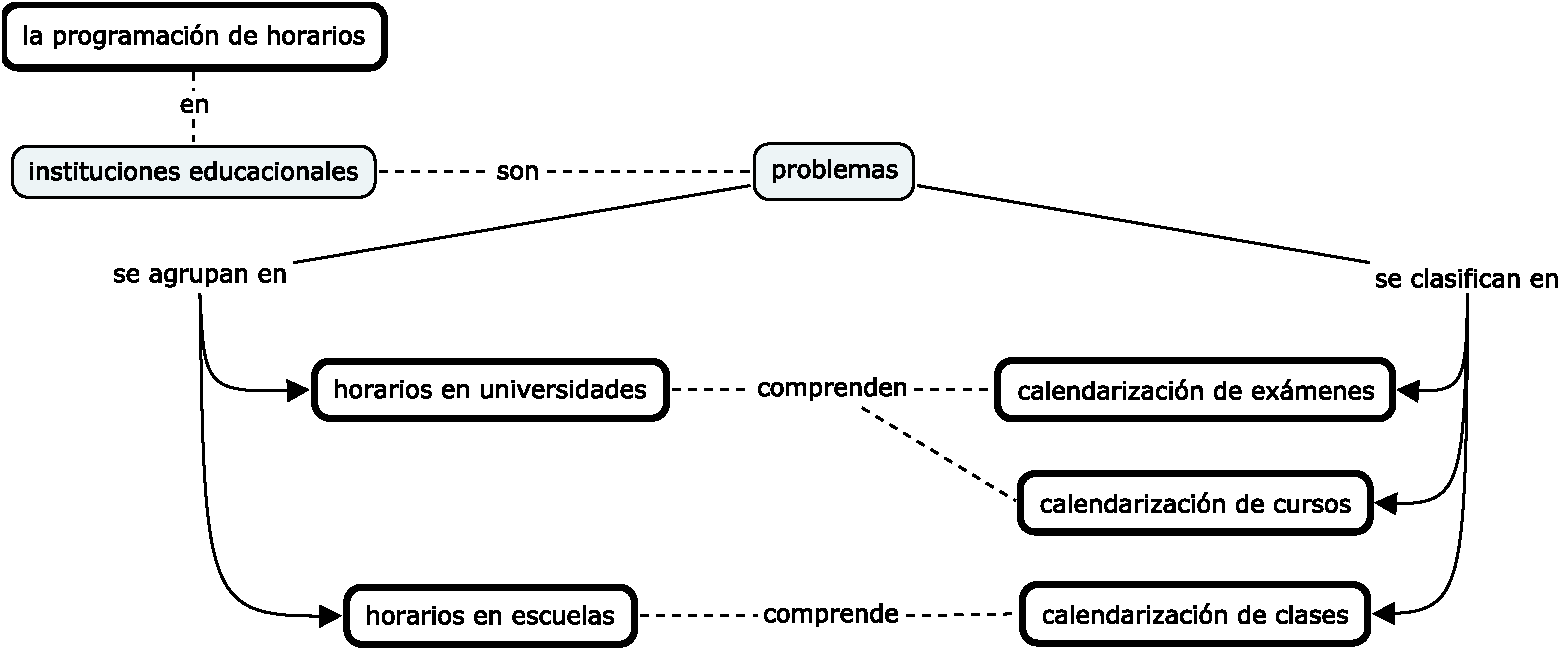
\includegraphics[width=.8\textwidth, trim=0 140 0 140]{timetabling_classification.pdf}
\caption[Clasificación del problema]{Clasificación de los problemas en la elaboración de horarios educacionales}
\label{fig:timetabling_classification}
\end{figure}

\iffalse
Classification of Educational Timetabling Problems
Schaerf (1999a) classified educational timetabling into three main classes i.e. school timetabling, course timetabling and examination timetabling. They share the same basic characteristics of the general timetabling problem but can still have significant differences between them. Each one of them has its own constraints, requirements and rules. More details on educational timetabling can be found in Burke et al. (2004e). In this section, a classification of educational timetabling and its properties are discussed. We divided educational timetabling into two categories i.e. school timetabling and university timetabling (which consists of examination timetabling and course timetabling).
\fi

\subsection{Horarios en escuelas}

\index{horarios!en escuelas}

\subsubsection{Horarios de clases}

\index{horarios!de clases}
De acuerdo a \citet[p.~88]{schaerf99a-survey-of-automated} el problema de horarios de clases consiste en calendarizar en un periodo semanal todas las clases de una escuela, evitando que los profesores se encuentren con dos clases al mismo tiempo, y viceversa. \citet[p.~10,11]{abdullah06heuristic-approaches} elabora explicando que el problema consiste de un conjunto de profesores, clases, lecciones y periodos semanales. En donde tales periodos semanales son predefinidos.

El problema intenta asignar lecciones a periodos y, un profesor a una clase en particular en un momento dado mientras se satisface un conjunto de limitaciones con el fin producir un horario factible. Algunos ejemplos de limitaciones en este tipo de problemas son las capacidades de alojamiento, ubicaciones, cargas de trabajo de los profesores, tiempo de descanso entre lecciones.

\iffalse
School timetabling: The weekly scheduling for all the classes of a school, avoiding teachers meeting two classes at the same time, and vice versa;

2.3.1 SchoolTimetabling
The school timetabling problem is concerned with the weekly scheduling for all the lessons of a school. The problem consists of a set of teachers, classes, subject/lessons and weekly periods. These weekly periods are predefined. This problem tries to assign lessons to periods and, a teacher to a particular class at a given time while satisfying a set of constraints in order to produce a feasible timetable. 

Some examples of constraints in the school timetabling problem are capacities, locations, teacher loads, rest time between two lessons and other personal preferences. Examples of research on school timetabling can be found in Abramson (1991) who employed simulated annealing, Carrasco and Pato (2001) who employed a multi- objective genetic algorithm and Legierski (2003) who applied a constraint-based approach.
\fi

\subsection{Horarios en universidades}

\index{horarios!en universidades}\index{calendarización!de cursos}\index{calendarización!de exámenes} 
El problema de la planificación de horarios en universidades puede ser agrupado en dos categorías: (i) calendarización de cursos y (ii) calendarización exámenes. 
El problema de la calendarización de cursos es el proceso de la asignación de periodos y aulas de manera tal que las reuniones entre conferenciantes y estudiantes pueda ocurrir. 
El problema de la calendarización de exámenes se refiere a la asignación de periodos y aulas de manera tal que los estudiantes puedan presentar sus exámenes. 
Ambos problemas son similares de manera superficial, pero existen diferencias importantes que los distinguen. 
En la calendarización de exámenes, múltiples exámenes pueden ser presentados en una misma aula (ej. auditorio) al mismo tiempo. 
Sin embargo, esto no es posible para la calendarización de cursos en donde únicamente un curso puede ser asignado a un aula \citep[p.~11]{abdullah06heuristic-approaches}.

\iffalse
The university timetabling problem can be grouped into two categories: (i) course (or lecture) timetabling and (ii) examination timetabling. The course timetabling problem is the process of assigning timeslots and rooms so that meetings between lecturers and students can take place. The examination timetabling problem refers to the assignment of timeslots and rooms so that students can take examinations. These two (examination and course) timetabling problems are fairly similar in some superficial ways, but there are some distinct underlying differences between them. In examination timetabling, several examinations can be assigned to one (large) room at the same time. However, this is not possible for course timetabling where only one course can be assigned to one room.
\fi

\subsubsection{Calendarización de exámenes}

\index{calendarización!de exámenes}\index{calendarización!de cursos}
\citet[p.~4]{carter95recent-developments} definió el problema como la asignación de exámenes a un número limitado de periodos de manera tal que no existan conflictos o coincidencias. Los problemas de calendarización de cursos y exámenes son similares pero algunas diferencias relevantes según \citet[p.~159]{werra85an-introduction-to-timetabling} son:
\begin{enumerate}[a]
\item Existe generalmente un solo exámen por cada tema (mientras que hay varias exposiciones en un curso)
\item En la calendarización semanal de cursos, el objetivo principal es evitar conflictos (ej. la ocurrencia de que dos cursos elegidos por un mismo estudiante sean programados en el mismo periodo). Para los exámenes, generalmente se pide un máximo de un examen por día para cada estudiante o de ser posible, evitar la calendarización de exámenes en días consecutivos si el periodo de evaluación de exámenes lo permite.
\end{enumerate}
El problema de la calendarización de exámenes es muy común tanto en escuelas como en universidades. La asignación de los exámenes a los periodos está sujeta a un conjunto de limitaciones \citep[p.~12]{abdullah06heuristic-approaches}.

\iffalse
course sched- uling problems and exam scheduling problems were quite similar; bo:2 types could be formulated in terms of node coloring in a graph. There are in fact a few differences which should be underlined.
a) There is usually only one exam in each subject (while we had several lectures in a course). Exam graphs will so be generally smaller in size than course scheduling graphs.
b) In a weekly course schedvle, the only objec- tive is to avoid conflicts (i.e. the sJtuation where 2 courses chosen by a student are scheduled m ~he same period). For the exams, it is usua]iy required to have at most one exam per day for each student or even to avoid having exams on consecutive days if the time interval for exams atlows it.

Examination timetabling: The scheduling for the exams of a set of univer- sity courses, avoiding overlap of exams of courses having common students, and spreading the exams for the students as much as possible.

11Chapter 2. A Review of University Timetabling Problems and Approaches
Carter and Laporte (1996) defined the examination timetabling problem as:
“The assigning of examinations to a limited number of available time periods in such a way that there are no conflicts or clashes”
The examination timetabling problem is very common in both schools and universities. It is concerned with allocating a set of examinations, into a limited number of timeslots (periods), subject to a set of constraints. Carter et al. (1994) quoted that the basic challenge of examination timetabling is to schedule examinations over a limited number of timeslots so as to avoid conflicts and to satisfy a number of side constraints. In this case, the conflict is referred to as a hard constraint and side constraints are referred to as soft constraints.
\fi

\subsubsection{Calendarización de cursos}

\index{calendarización!de cursos}
El problema de la calendarización de cursos surge cuando una universidad (o incluso una escuela) ofrece una colección de cursos (cada uno consistiendo de un número dado de conferencias) sin existir un currículo fijo y en donde cada estudiante puede elegir cierto número de cursos. El problema consiste en la asignación de cada lectura a algún periodo en la semana de manera tal que ningún estudiante requiera asistir a más de una conferencia a la vez \citep[p.~157]{werra85an-introduction-to-timetabling}. 
\citet[p.~88]{schaerf99a-survey-of-automated} define el problema como la calendarización semanal de todas las lecciones de un conjunto de cursos universitarios, minimizando los empalmes de las lecciones de cursos teniendo estudiantes en común.

\iffalse
The course scheduling problem arises when a university (or even a school) offers a collection of courses (each one consisting of a given number of lectures) and there is no fixed curriculum: Each student may choose a certain number of courses. The problem consists in assigning each lecture to some period of the week in such a way that no student is required to take more than one lecture at a time. {werra85an-introduction-to-timetabling}

Course timetabling: The weekly scheduling for all the lectures of a set of university courses, minimizing the overlaps of lectures of courses having common students;{schaerf99a-survey-of-automated}
\fi

\section{Horarios de clases}

\section{Calendarización de cursos}

\section{Calendarización de exámenes}

\chapter{Preliminares}

\section{Introducción}

\section{Historia de la calendarización}

\section{Terminología y definiciones}

\section{Complejidad computacional}

\subsection{Clases P y NP}

\chapter{Modelos matemáticos}

\section{Introducción}

\section{planificación de horarios en escuelas}

\section{Calendarización de cursos}

\section{Calendarización de exámenes}

\section{Un lenguaje en común}

\section{Algoritmos de solución}

\chapter{Limitantes y funciones objetivo}

\section{Introducción}

\section{Limitantes}

\section{Funciones objetivo}

\chapter{El gestor escolar}

\section{Aplicaciones}

\subsection{Métricas de desempeño}

\subsection{Multidisciplinario}

\section{Factores de interés}

\subsection{Laborales}

\subsubsection{Regulatorios}

\subsection{Diagnóstico}

\subsubsection{Interinstitucional}

\subsection{Inversión}

\subsubsection{Downsizing}

\subsection{Económicos}

\subsubsection{Utilidades}

\subsubsection{Fiscales}

\subsubsection{Aprovechamiento de recursos}

\subsection{Sociales}

\subsubsection{Involucramiento de paterfamilias}

\subsection{Institucionales}

\subsubsection{Profesorado}

\subsection{Flexibilidad}

\chapter{Herramientas de solución}

\section{Tipo de herramientas}

\subsection{Automatizadas}

\subsection{Interactivas}

\section{Listado de software}

\subsection{KHE}

\subsubsection{Formato de datos}

\chapter{Trabajo en el futuro y conclusiones}

\section{Resumen del trabajo de investigación}

\section{Contribuciones}

\section{Trabajo futuro}

\section{Diseminación}

\index{timetabling!university|see{planificación de horarios en universidades}}
\index{timetabling!school|see{horarios de clases y planificación de horarios en escuelas}}
\index{timetabling!course|see{calendarización de cursos}}
\index{timetabling!examination|see{calendarización de exámenes}}

\index{scheduling|see{planificación}}
\index{timetabling|see{planificación de horarios}}

% Bibliography
\bibliographystyle{apalike}
\bibliography{/Users/harciga/Dropbox/bibliographies/reviewed}
\bibliography{/Users/harciga/Dropbox/bibliographies/Dissertation books}
{
\RaggedRight
\printindex
}
\end{document}
